\documentclass{article} % Change to the appropriate document class, i.e. report, book, article...
\usepackage{style}

\title{CSE 272 assignment 1}
\author{Alisha Lawson\\Hallgeir Lien}
\date{}
\begin{document}

\maketitle
\newpage

\section*{Introduction}
In this assignment we explore different methods of estimating the irradiance at a point in a scene. The scene used for the assignment has a square diffuse area light with corners $(-1,10,-1)$ and $(1,10,1)$ (area $A=4\ m^2$)and normal $(0,-1,0)$ and power $100\ W$, a mirror with corners $(5,4,-1)$ and $(5,6,1)$ and normal $(-1,0,0)$, and a plane with origin $(0,0,0)$ and normal $(0,1,0)$. We will estimate the irradiance at the point $A=(0,0,0)$ using path tracing, progressive photon mapping and a combination of path tracing and area light sampling with multiple importance sampling.

\section*{Task 1}
Our first task was to estimate the irradiance using path tracing. We shot out up to 1 million rays from the point A, with a probability distribution of $p_P(x) = \cos \theta / \pi$, where $\theta$ is the angle between the normal at $A$ and the ray direction. The results are plotted in figure \ref{fig:pathtracing}. 
\begin{figure}[h]
\begin{tabular}{c}
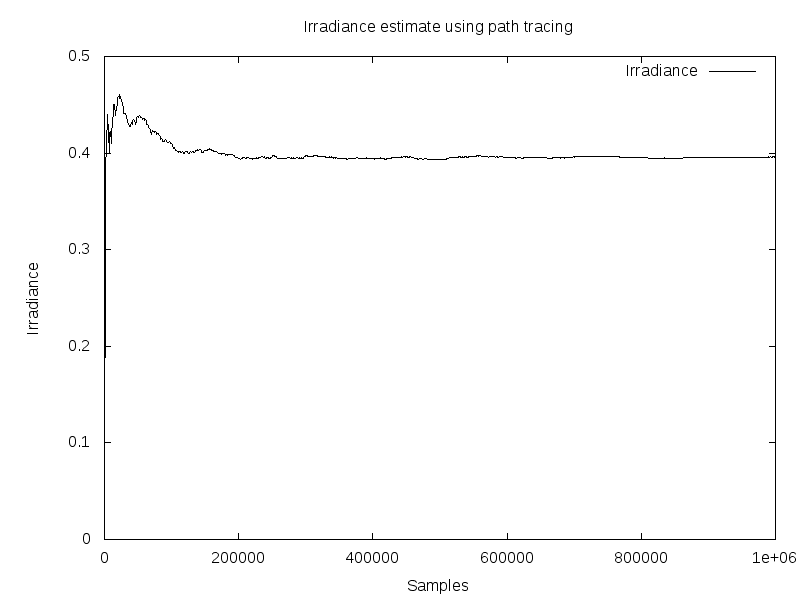
\includegraphics[width=0.9\textwidth]{plots/irrad_pathtracing.png}\\
\end{tabular}
\caption{Irradiance estimate, path tracing}
\label{fig:pathtracing}
\end{figure}

We calculate the irradiance by summing over all the contributions and averaging:
$$F=\frac{1}{N}\sum_{i=1}^N \frac{f(x)}{p_P(x)} = \frac{\pi}{N}\sum_{i=1}^N \frac{f(x)}{\cos \theta_o}\ W/m^2$$
$f(x) = 0$ if the sample ray misses the light source, and $f(x) = (\Phi/(\pi\cdot A))\cdot \cos \theta_i$. Note that for this scene, the incident angle to the light's surface and outgoing angle from the point A is identical and cancels out, and that the power per area is $25\ W/m^2$, so the above estimate simplifies to 
$$F=\frac{\pi}{N}\sum_{i=1}^N 25\ W/m^2$$
The estimate seems to converge to a point near $F=0.39$ for the scene above. 

\section*{Task 2}
Our second task was to estimate the irradiance using Progressive Photon mapping.  We sent out 100,000 photons for 1,000 passes totaling 100 million photons emitted from the square light, which has a normal bias distribution. Initially we set the radius to $0.25$. On each pass we adjust the radius $\hat{R}(x)$ according the user-defined ratio alpha $\alpha$ set to 0.7, as
$$ \hat{R}(x) = R(x) - dR(x) = R(x)\sqrt{\frac{N(x)+\alpha M(x)}{N(x)+M(x)}}$$
Where $N(x)$ is the previously accumulated photons and $M(x)$ is the newly added photons in the current photon tracing pass for each hitpoint in the scene. Figure \ref{fig:pm_radius} shows the radius and figure \ref{fig:pm_acc} shows the number of accumulated photons over 1,000 iterations.

\begin{figure}[H]
\begin{tabular}{c}
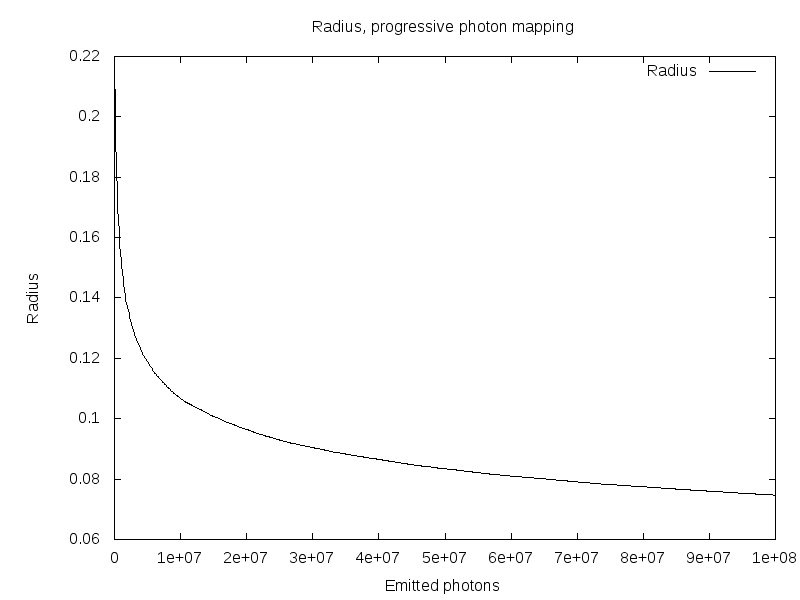
\includegraphics[width=0.9\textwidth]{plots/irrad_photonmap_radius.png}\\
\end{tabular}
\caption{Radius, photon mapping}
\label{fig:pm_radius}
\end{figure}

\begin{figure}[h]
\begin{tabular}{c}
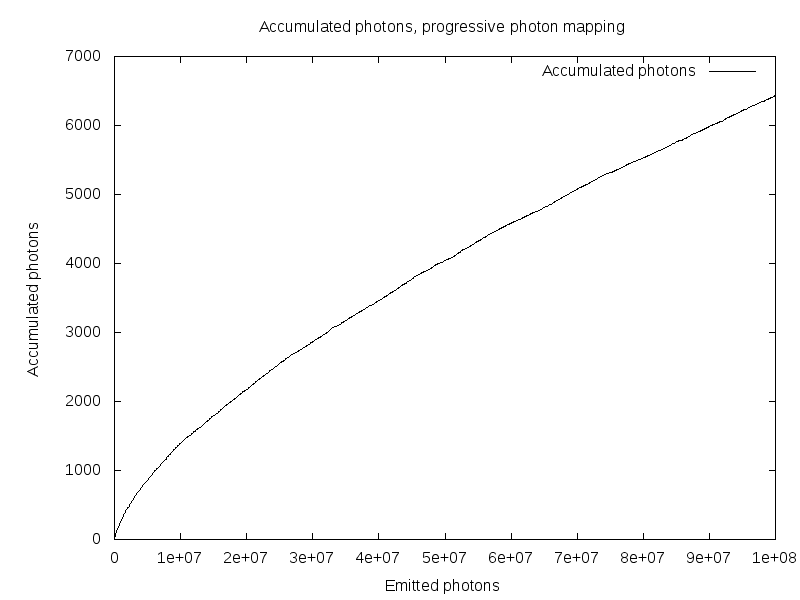
\includegraphics[width=0.9\textwidth]{plots/irrad_photonmap_photons.png}\\
\end{tabular}
\caption{Accumulated photons}
\label{fig:pm_acc}
\end{figure}

We also modify the accumulated flux $\tau_{\hat{N}}(x, \omega)$ in each pass, using
$$\tau_{\hat{N}}(x, \omega) = \tau_{N+M}(x, \omega)\frac{N(x) + \alpha M(x)}{N(x) + M(x)}$$

Since we are interested in the irradiance at point A, the BRDF does not contribute to the equation. We calculate the irradiance by normalizing $\tau_{\hat{N}}(x, \omega)$ by the number of emitted photons and the adjusted radius $\hat{R}(x)$:
$$F = \frac{\tau_{N}(x, \omega)}{\pi R(x)^2 N_{emitted}}$$

\begin{figure}[H]
\begin{tabular}{c}
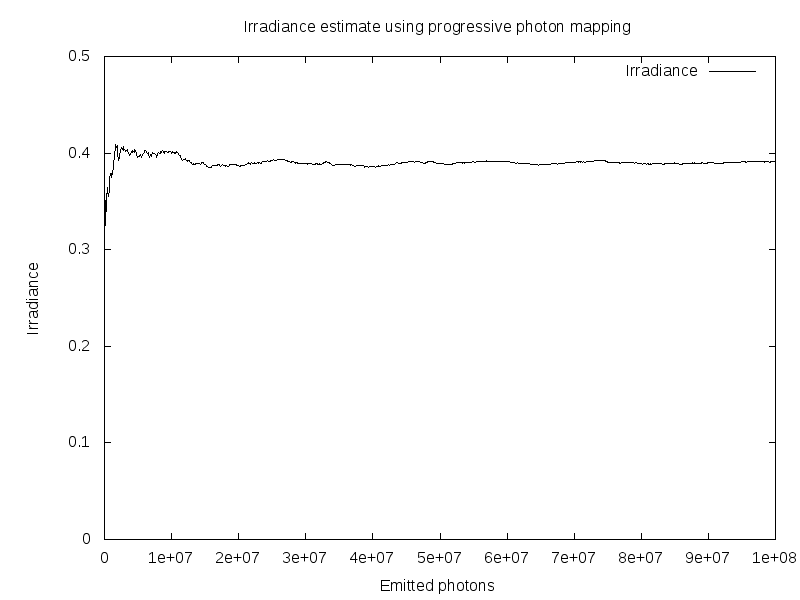
\includegraphics[width=0.9\textwidth]{plots/irrad_photonmap.png}\\
\end{tabular}
\caption{Irradiance, photon mapping}
\label{fig:pm_irradiance}
\end{figure}

Over multiple photon tracing passes the irradiance also converges to about 0.39, as with path tracing.

\section*{Task 3 - Multiple importance sampling}
In the third task we would estimate the irradiance by combining both area light sampling and path tracing using multiple importance sampling with the balance heuristic
$$
F = \frac{1}{N}\sum_{i=1}^n \sum_{j=1}^{n_i} \frac{f(x)}{\sum_k n_k/N \cdot p_k(x)}
$$
where $N$ is the total number of samples, $n_i$ is the number of samples taken with method $i$, $f(x)$ is the sample value and $p_k(x)$ is the probability of shooting a ray in the direction of $x$ using the probability distribution $p_k$. Figure \ref{fig:importance} shows the irradiance estimate as the number of samples increases. 

The area samples was gathered by choosing a random point on the area light surface with $p_A(x)=1/A$, then evaluating
$$
f(x) = \frac{25}{\pi} \cdot \frac{\cos^2 \theta}{||x-x^\prime||^2}
$$

The path tracing samples was gathered like in task 1.

\begin{figure}[h]
\begin{tabular}{c}
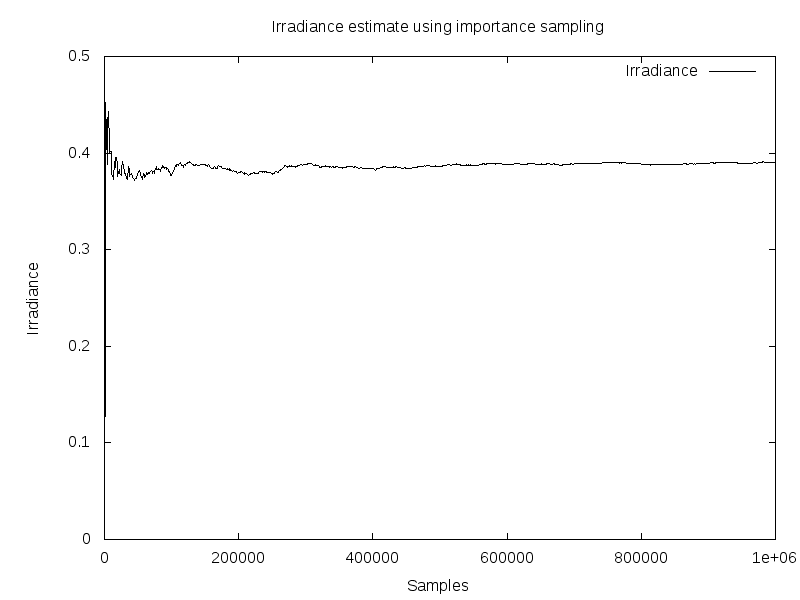
\includegraphics[width=0.9\textwidth]{plots/irrad_importance.png}\\
\end{tabular}
\caption{Irradiance estimate, importance sampling}
\label{fig:importance}
\end{figure}

As we see, even though the variance is quite high in the beginning, the estimate seems to drop to and fluctuate around $0.39$ after just a few samples, where the pure path tracing approach overestimated the irradiance for the first 200000 samples.

\end{document}
